\documentclass[tikz,border=2pt]{standalone}
\usepackage{amsmath}
\usepackage{pgfplots}
\pgfplotsset{compat=1.18}

\begin{document}
% The domain is the set of inputs for which f is defined: for f(x)=sqrt(4-x^2) it is [-2,2],
% the shadow of the graph on the x-axis.
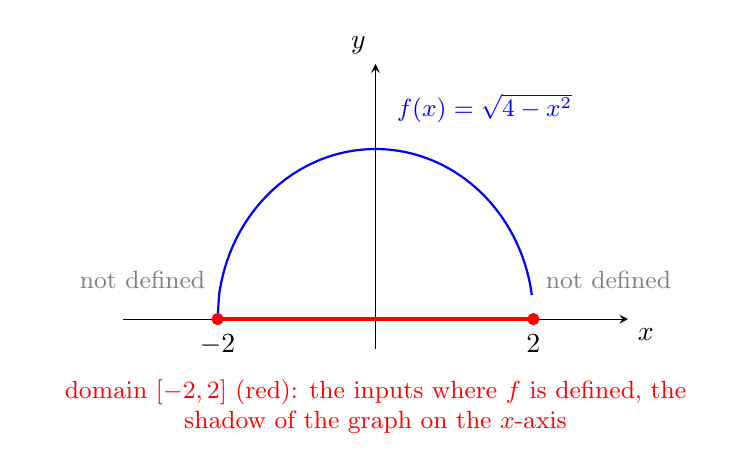
\begin{tikzpicture}
	\begin{axis}[
		axis lines=middle,
		xmin=-3.2, xmax=3.2,
		ymin=-0.35, ymax=3.0,
		xtick={-2,2}, ytick=\empty,
		xlabel={$x$}, ylabel={$y$},
		xlabel style={below right}, ylabel style={above left},
		samples=200, smooth, clip=false,
		width=8cm, height=5.2cm
		]
		\addplot[thick, blue, domain=-2:2] {sqrt(4-x^2)};
		\draw[very thick, red] (axis cs:-2,0) -- (axis cs:2,0);
		\addplot[only marks, mark=*, red] coordinates {(-2,0) (2,0)};
		\node[blue, anchor=south west, font=\small] at (axis cs:0.15,2.2) {$f(x)=\sqrt{4-x^2}$};
		\node[gray, anchor=south, font=\small] at (axis cs:-2.95,0.25) {not defined};
		\node[gray, anchor=south, font=\small] at (axis cs:2.95,0.25) {not defined};
	\end{axis}
	\node[red, anchor=north, font=\small, align=flush center, text width=8.6cm] at ([yshift=-2pt]current axis.outer south) {domain $[-2,2]$ (red): the inputs where $f$ is defined, the shadow of the graph on the $x$-axis};
\end{tikzpicture}
\end{document}
